\documentclass{article}

% if you need to pass options to natbib, use, e.g.:
%     \PassOptionsToPackage{numbers, compress}{natbib}
% before loading neurips_2026
\PassOptionsToPackage{numbers,compress}{natbib}

% The authors should use one of these tracks.
% Before accepting by the NeurIPS conference, select one of the options below.
% 0. "default" for submission
\usepackage[dblblindworkshop]{neurips_2026}
% the "default" option is equal to the "main" option, which is used for the Main Track with double-blind reviewing.
% 1. "main" option is used for the Main Track
%  \usepackage[main]{neurips_2026}
% 2. "position" option is used for the Position Paper Track
%  \usepackage[position]{neurips_2026}
% 3. "eandd" option is used for the Evaluations & Datasets Track
% \usepackage[eandd]{neurips_2026}
% 4. "creativeai" option is used for the Creative AI Track
%  \usepackage[creativeai]{neurips_2026}
% 5. "sglblindworkshop" option is used for the Workshop with single-blind reviewing
% \usepackage[sglblindworkshop]{neurips_2026}
% 6. "dblblindworkshop" option is used for the Workshop with double-blind reviewing
%  \usepackage[dblblindworkshop]{neurips_2026}
% 7. "education" option is used for the Education Track
%  \usepackage[education]{neurips_2026}

% "preprint" option is used for arXiv or other preprint submissions
% \usepackage[preprint]{neurips_2026}

% to avoid loading the natbib package, add option nonatbib:
%    \usepackage[nonatbib]{neurips_2026}

%% ---- packages loaded by the NeurIPS 2026 template, in template order ----
\usepackage[utf8]{inputenc} % allow utf-8 input
\usepackage[T1]{fontenc}    % use 8-bit T1 fonts
\usepackage{hyperref}       % hyperlinks
\usepackage{url}            % simple URL typesetting
\usepackage{booktabs}       % professional-quality tables
\usepackage{amsfonts}       % blackboard math symbols
\usepackage{nicefrac}       % compact symbols for 1/2, etc.
\usepackage{microtype}      % microtypography
\usepackage{xcolor}         % colors

%% ---- additional packages this paper needs ----
\usepackage{amsmath,amssymb,bm}
\usepackage{graphicx}
\usepackage{tikz}
\usetikzlibrary{arrows.meta}
\usepackage{cleveref}       % must be loaded after hyperref

% Note. For the workshop paper template, both \title{} and \workshoptitle{} are required, with the former indicating the paper title shown in the title and the latter indicating the workshop title displayed in the footnote. 
\workshoptitle{WORKSHOP TITLE}
\title{Variational inference in coupled models of amino acid substitution}

% The \author macro works with any number of authors. There are two commands
% used to separate the names and addresses of multiple authors: \And and \AND.
%
% Using \And between authors leaves it to LaTeX to determine where to break the
% lines. Using \AND forces a line break at that point. So, if LaTeX puts 3 of 4
% authors names on the first line, and the last on the second line, try using
% \AND instead of \And before the third author name.


\author{%
	Annabel Large \\
	Department of Bioengineering\\
	University of California, Berkeley\\
	Berkeley, CA 94720, USA \\
	\texttt{annabel\_large@berkeley.edu} \\
	\And
	Ian Holmes \\
	Department of Bioengineering\\
	University of California, Berkeley\\
	Berkeley, CA 94720, USA \\
	\texttt{ihh@berkeley.edu} \\
}


%% ---- EXTRA (not from NeurIPS template): custom commands ----
\newtheorem{defn}{Definition}
\newtheorem{rem}{Remark}
\crefname{defn}{Definition}{Definitions}
\Crefname{defn}{Definition}{Definitions}
\crefname{rem}{Remark}{Remarks}
\Crefname{rem}{Remark}{Remarks}

\graphicspath{{./figures/}}

\newcommand{\TKF}{\textsc{TKF}}
\newcommand{\CTBN}{\textsc{ctbn}}
\newcommand{\CTMC}{\textsc{ctmc}}
\newcommand{\EM}{\textsc{em}}
\newcommand{\Reversible}{\textsc{Reversible}}
\newcommand{\Coupledm}{\textsc{Coupled}}
\newcommand{\Exchm}{\textsc{Exchangeable}}
\newcommand{\Metrop}{\textsc{Metropolis}}
\newcommand{\DCA}{\textsc{dca}}
\newcommand{\Pfam}{\textsc{Pfam}}
\newcommand{\E}{\mathbb{E}}
\newcommand{\R}{\mathbb{R}}
\newcommand{\Xset}{\mathcal{A}}
\newcommand{\partition}{\mathcal{P}}
\newcommand{\Clus}{\mathrm{Clus}}
%\newcommand{\Lumpm}{\textsc{Lumpable}} 
%\newcommand{\Halflump}{\textsc{Half-lumpable}} 
%\newcommand{\TKFDP}{\textsc{TKF--DP}} 


\begin{document}

\maketitle

\begin{abstract}
We investigate the use of Expectation--Maximization (\EM) and variational Bayes for inferring rates and interactions under
models of molecular coevolution.
We first review \EM\ theory for continuous-time Markov chains (\CTMC s) and develop it for coevolutionary models,
exploiting exchangeability and reversibility symmetries to constrain the parameter dimension.
We fit several paired amino-acid coevolutionary models to structural alignments
and compare the results to previous work.
Our richest model trained on pooled coevolutionary data has explanatory power comparable to CherryML's Q2 matrix (also trained on pooled data), with half the parameters.
However, we observe that aggregation of training data can lead to a form of Simpson's Paradox: a mixture model,
whose components are parameter-efficient continuous-time Bayes networks (\CTBN s),
resolves signals that wash out when a single model tries to capture everything.
These signals include both correlated and anticorrelated hydropathy and volume-packing in coevolving amino-acid pairs,
as well as the anticorrelated acid/base compensation that was detected by CherryML's Q2.
We next present an evidence lower bound (ELBO) for \CTBN s built from the same \EM\ statistics, in which the coupling
contracts onto per-site bridge quantities at a cost polynomial, rather than exponential, in cluster size.
Compared to the state of the art in variational modeling of \CTBN s, the Euler-Lagrange equations derived by Cohn et al (JMLR, 2010),
it is competitive in accuracy, considerably more efficient, simpler, and better conditioned:
closed-form for coupled pairs, and for larger clusters analytic where theirs is singular at the branch endpoints.
%%% removing tkf-dp
%We conclude by describing a covariant indel model: a Dirichlet process
%selecting coevolving sites within TKF92, yielding an Infinite
%Pair HMM over alignments and structures. This model slightly outperforms TKF92 on a
%structural-alignment benchmark. 
\end{abstract}

%% The NeurIPS 2026 template has no keywords element, so these are
%% commented out rather than dropped:
%% Keywords: coevolution; continuous-time Markov chain; reversibility;
%% exchangeability; lumpability; Potts model; Dirichlet process; TKF model.

% =============================================================
\section{Introduction}
\label{sec:intro}
% =============================================================

A protein's three-dimension structure imposes biophysical constraints that modulate selection on its amino acid sequence.
These constraints cause substitution rates to vary between sites; for example, hydrophobic cores tolerate fewer mutations and evolve more slowly.
Residues in three-dimensional contact are also observed to co-evolve, a phenomenon known as epistasis.
An expressive model of sequence coevolution should mechanistically account for both substitution rate heterogeneity and epistatic interactions.
Building such models requires designing suitable parameterizations, efficient methods for likelihood computation and model fitting, and tractable algorithms for sequence alignment and phylogenetic inference.

% need to double-check these method descriptions
Standard substitution models assume residues evolve independently. 
To account for coevolution, context- and neighbor-dependent substitution models relax the site-independence assumption~\cite{ArndtBurgeHwa2003NeighborDependent,JensenPedersen2000ContextDependent,LunterHein2004NearestNeighbor,SiepelHaussler2004ContextML}.
However, exact likelihood computation under these models becomes challenging.
Proposed inference strategies include MCMC-EM and pseudolikelihood 
methods~\cite{ChristensenHobolthJensen2005PseudoLikelihood,Hobolth2008MCMCEM}, 
variational approximations and likelihood bounds~\cite{cohn2010,JojicEtAl2004PhyloHMM,MatsenRalph2022BoundingDependency,WexlerGeiger2007VariationalUpper}, 
and importance sampling~\cite{MathewsSchmidler2025ImportanceSampling}. 

Our work builds upon several specific methodological advances from this literature.
General expectation-maximization (EM) methods for continuous-time Markov 
chains (\CTMC s) use endpoint-conditioned sufficient statistics to estimate substitution 
rates~\cite{HolmesRubin2002,HobolthJensen2005,HobolthJensen2011}. 
CherryML accelerates gradient-based parameter estimation for substitution models by using discretized 
branch lengths and a composite likelihood over the closest pairs of leaves in a phylogenetic tree (i.e. "cherries")~\cite{Prillo2023CherryML}. 
\citet{cohn2010} used variational calculus to derive an evidence lower bound (ELBO) for continuous-time Bayesian networks (\CTBN s).
Finally, the CAT model\cite{Lartillot2004} uses Dirichlet processes to assign parameters to mixtures of substitution models.
 We adapt and extend these ideas to develop tractable models of sequence coevolution.

In \Cref{sec:single}, we first review independent-site substitution models, their accompanying expectation-maximization algorithm, and two common modeling assumptions (exchangeability and reversibility).
We then consider models that explicitly include interactions between pairs of sites (\Cref{sec:pair} and derive new EM algorithms to account for varying exchangeability and reversibility assumptions. 
In \Cref{sec:paircompare}, we evaluate variants of pairwise models against prior work, including CherryML~\cite{Prillo2023CherryML}. 
Finally, we present a new closed-form ELBO for multi-site models. In our evaluations, this form is more stable than the~\citet{cohn2010} ODE-based ELBO (\Cref{sec:multi}).
%Finally (\Cref{sec:tkfdp}), we describe how the various symmetries we have outlined can be used to add covariation to the TKF92 indel model~\cite{ThorneEtAl92}.

% =============================================================
\section{Single-site models}
\label{sec:single}
% =============================================================
%%% TODO: maybe change x and y to i and j? It's confusing when you move to the paired site models
A single site evolves from $x$ to $y$ ($x,y \in \Xset$, the sequence alphabet) as a continuous-time Markov chain (\CTMC) with generator $Q$, equilibrium distribution $\pi$, off-diagonal rates $Q_{xy}\ge0$,
$Q_{xx}=-\sum_{y\ne x}Q_{xy}$, and stationary $\pi Q=0$. We keep the chain
reversible, $\pi_xQ_{xy}=\pi_yQ_{yx}$, so the symmetrized matrix
$\widetilde Q_{xy}=Q_{xy}\sqrt{\pi_x/\pi_y}$ is real with
spectral decomposition $\widetilde Q=\sum_k\xi_k v^{(k)}{v^{(k)}}^\top$,
$\xi_k\le0$. Conjugating back gives the branch transition matrix,
\begin{equation}
\label{eq:pt}
P(t)_{xy}=\big(e^{Qt}\big)_{xy}=\sqrt{\pi_y/\pi_x}\;\textstyle\sum_k
   e^{\xi_k t}\,v^{(k)}_x v^{(k)}_y,
\end{equation}
and the tree likelihood is the sum-product recursion of Felsenstein
pruning~\cite{Felsenstein81}
The generalized time-reversible (GTR,~\cite{tavare1986some}) parameterization writes
$Q_{xy}=S_{xy}\,\pi_y$ with $S=S^\top$ exchangeabilities, so spectral decomposition
$\widetilde Q_{xy}=S_{xy}\sqrt{\pi_x\pi_y}$. LG08~\cite{LG08} is one such parameterization of $S$.

\paragraph{The E-step.} The sufficient statistics of a branch
trajectory $\mathbb X=(X(u))_{0\le u\le t}$ are the dwell times $W_x$ and
transition usages $U_{xy}$. The complete-data log-likelihood is
\begin{equation}
\label{eq:cdl}
\ell(Q)=\log P(\mathbb X\mid X(0),Q)=\sum_{x\ne y}U_{xy}\log Q_{xy}
   -\sum_x W_x\!\!\sum_{y\ne x}\!Q_{xy}.
\end{equation}
The endpoint-conditioned expectations of the sufficient statistics are~\cite{HobolthJensen2005,HobolthJensen2011,HolmesRubin2002},
\begin{equation}
\label{eq:bridge}
\E[W_x\mid a,b]=\frac{I^{ab}_{xx}(t)}{M_{ab}(t)},\qquad
\E[U_{xy}\mid a,b]=\frac{Q_{xy}\,I^{ab}_{xy}(t)}{M_{ab}(t)},
\end{equation}
with the matrix exponential $M(t)=e^{Qt}$ and its time convolution $I^{ab}_{xy}(t)=\int_0^t M_{ax}(u)\,M_{yb}(t{-}u)\,du$.
% AL: does this need to be introduced at all?
To evaluate the time convolution, we use the following exponential divided-difference kernel:
\begin{equation}
\label{eq:bridgestat}
J^{kl}(t)=
\begin{cases}(e^{\xi_k t}-e^{\xi_l t})/(\xi_k-\xi_l)&\xi_k\ne\xi_l,\\[2pt]
t\,e^{\xi_k t}&\xi_k=\xi_l.\end{cases}
\end{equation}

\paragraph{The M-step.} This step depends on the substitution model parameterization.
For example, under GTR, letting $V_x$ count the ancestral state
(the event $X(0)=x$) and $V'_x=V_x+\sum_{y\ne x}U_{yx}$, the
complete-data log-likelihood including the root is
\begin{equation}
\label{eq:ell2}
\ell(S,\pi)=\sum_x V'_x\log\pi_x+\sum_{y>x}(U_{xy}{+}U_{yx})\log S_{xy}
 -\sum_{y>x}S_{xy}\big(W_x\pi_y+W_y\pi_x\big).
\end{equation}
The joint equations for $(S,\pi)$ are nonlinearly coupled with no closed form.
Therefore, the two parameter blocks must be updated iteratively.
Fixing $\pi$, the exchangeabilities $S$ have the closed-form maximizer
$\widehat S_{xy}=(U_{xy}{+}U_{yx})/(W_x\pi_y+W_y\pi_x)$. 
There is no canonical optimization for the $\pi$ update step, though several strategies have been proposed.
One option is to fix $\pi\propto V'$ and only fit $S$.
Alternatively, since the $\pi$ parameter block is strictly concave on the simplex at fixed $S$, the two parameter blocks can be fitted through iterative conditional updates.
A fixed-point $\pi$ update is recovered by a \emph{secret-destination augmentation} (originally proposed in~\citet{Bruno1996}).
From state $x$, a move is proposed with rate $S_{xy}$, a hidden token is drawn from $\pi$, and the move is accepted only if the hidden token is $y$.
The $\pi$-dependence of the augmented complete data likelihood now arises entirely from tokens drawn from $\pi$:
the root state, the substitution counts $\sum_{y}U_{yx}$ (together, $V'_x$), and the latent tokens of the rejected attempts,
whose expected count is $V''_x = \pi_x( W_x R_x + \sum_{y\ne x} W_y(R_y-S_{yx}) )$ with $R_y=\sum_{z\ne y}S_{yz}$.
The augmented counts are multinomially-distributed; the conjugate Dirichlet is maximized by $\widehat\pi_x\propto V'_x+V''_x$,
iterated to convergence.

%\paragraph{Symmetric parameterisation.} The same reversible chain is
%$Q=D^{-1/2}\Lambda D^{1/2}$ with $D=\mathrm{diag}(\pi)$ and
%$\Lambda=\Lambda^\top$, the form the pair model of \Cref{sec:pair}
%generalises.

%\paragraph{The three single-site symmetries.} All symmetries are
%artificial, and some are useful as null hypotheses. \emph{Reversibility}
%%is the one above. \emph{Uniformity} treats residues as interchangeable
%apart from their frequencies, and is what an aggregated model such as
%Jukes--Cantor or Kimura's two-parameter chain imposes. \emph{Strand
%complementarity} constrains nucleotide chains so the two strands evolve
%alike. Imposing a symmetry reduces parameters but, except for simple
%aggregation, complicates fitting by adding equations to solve rather than
%by giving a closed form.

%\paragraph{Exchangeability and site classes.} Exchangeability sits in the
%background of the single-site model and moves to the centre as sites
%couple. It is the statement that residue identity matters only through
%permutation-invariant labels. Site classes enter even here as the device
%that retains differentiated site identity under exchangeability: a
%Dirichlet process over background compositions, as in
%CAT-DP~\cite{Lartillot2004}, assigns each column one of a set of
%equilibrium distributions $\pi^{(c)}$, and averages over which columns
%share a class. CAT-DP is a prior on the class labels of an otherwise
%time-homogeneous model, and changes none of the mechanics above. As sites
%couple, the same class labels become the handle through which coupling
%acts.

% =============================================================
\section{Two-site models}
\label{sec:pair}
% =============================================================
\subsection{The smallest two-site model: a pair of telegraph processes}
\label{sec:pairbinary}
We illustrate the coupled substitution models with a simple example: a pair of telegraph processes.
Consider two binary components $x,y\in\{0,1\}$ evolving on the state space $00,01,10,11$ (Figure~\ref{fig:params}).
The flux has twelve parameters; the reversibility constraint leaves six free parameters (the \Reversible\ model).
The flux exchangeability constraint further reduces the parameter count to four (the \Exchm\ model).
We then consider asynchronous models, a specialization that forbids simultaneous flips.
The most general asynchronous coupled telegraph has two free rate parameters (the \Coupledm\ model). 
Fixing the proposal (the \Metrop\ model) leaves only one rate to determine the time scale.
The stationary distribution starts with four probability parameters; the normalization and stationary exchangeability ($\pi_{01} = \pi_{10}$) constraints each remove a degree of freedom, leaving two free parameters that correspond to mean and covariance.

%%% end of paragraph, before removing lumps:
%We then consider two different kinds of specialization: the asynchronous models, which forbid simultaneous flips, and the lumpable models, which must use them.
%The most general asynchronous coupled telegraph has two free rate parameters (\Coupledm); fixing the proposal (\Metrop) leaves only one rate to determine the time scale.
%Conversely, lumpability --- the property that the chain stays Markovian if projected onto a single component --- forces the chain to use simultaneous transitions to model correlations between the components.
%A non-exchangeably lumpable model is projectable onto the first component only (\Halflump); the exchangeable version is projectable onto both components (\Lumpm).
%Comparing the asynchronous models (\Coupledm, \Metrop) with the synchronized models (\Halflump, \Lumpm), the asynchronous ones are both favored by the data and significantly easier to train.


% \subsection{Example: a Watson--Crick base pair}
% \label{sec:pairdna}
% %The nucleotide case is the rung between the binary telegraph and the
% %$A{=}20$ chain, and it isolates one lesson cleanly: lumping a coupled
% %process pushes the coupling into the single-site \emph{margin}.
% Two paired nucleotides $x,y\in\{A,C,G,T\}$ substitute by an asynchronous
% single-site proposal with no transition/transversion structure (JC69),
% Metropolis-reweighted by a Potts energy supported only on the three
% base-pair edges,
% \[
%   E(i,j)=E_{at}\ \text{on}\ \{A,T\},\quad E_{cg}\ \text{on}\ \{C,G\},
%   \quad E_{gt}\ \text{on}\ \{G,T\},\quad 0\ \text{otherwise},
% \]
% with $\pi(i,j)\propto q(i)q(j)e^{-E(i,j)}$ (a favoured pair has lower
% energy). %The one structural fact that matters: all three bonds are
% %purine--pyrimidine pairs, so the energy sits entirely on
% %\emph{transversion} edges, while the two transition edges A--G and C--T
% %carry none.
% 
% The single-site marginal of this coupled chain is not itself Markov, but
% its best single-component (partner-marginalised) generator
% $W_{\mathrm{eff}}$ is exactly a reversible GTR chain. Writing
% $\alpha=e^{-E_{at}/2}$, $\gamma=e^{-E_{cg}/2}$, $\omega=e^{-E_{gt}/2}$, its
% stationary transition/transversion flux ratio is %has the closed form
% \[
%   \kappa_{\mathrm{ts/tv}}-1
%   \;=\;\frac{(2-\alpha-\gamma)(1-\omega)}{2\,(1+\alpha+\gamma+\omega)}.
% \]

\subsection{The general pair chain}
\label{sec:pairgeneral}

\begin{figure}[t]
\centering
%% Single row of four panels with the caption alongside, to save vertical space.
%% \resizebox scales the text with the cells, leaving internal proportions as drawn.
\begin{minipage}[c]{0.62\textwidth}
\resizebox{\textwidth}{!}{%
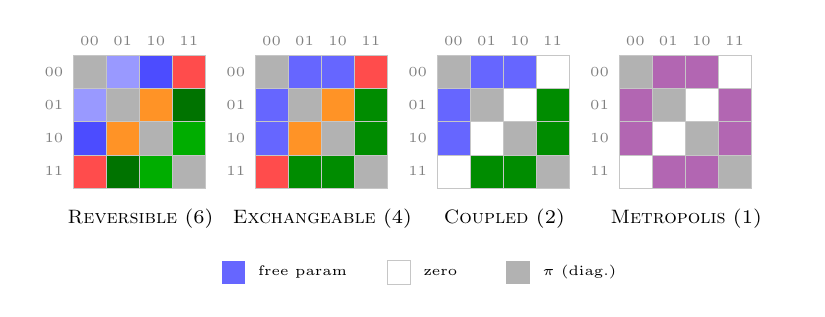
\begin{tikzpicture}[x=0.42cm,y=0.42cm,font=\scriptsize,
   cell/.style={draw=gray!45,line width=0.2pt}]
% row-major cells per panel: 00[pi,e1,e2,e5] 01[e1,pi,e6,e3] 10[e2,e6,pi,e4] 11[e5,e3,e4,pi]
\newcommand{\pnl}[4]{\begin{scope}[shift={(#1,#2)}]
  \foreach \col [count=\ii from 0] in {#4}{
     \pgfmathtruncatemacro{\rr}{3-int(\ii/4)}\pgfmathtruncatemacro{\cc}{mod(\ii,4)}
     \fill[\col] (\cc,\rr) rectangle ++(1,1);\draw[cell] (\cc,\rr) rectangle ++(1,1);}
  \node[anchor=north,align=center,text width=2.6cm] at (2,-0.35){#3};
  % state labels on both axes of every panel
  \foreach \s [count=\k from 0] in {11,10,01,00}{\node[left,gray] at (0,\k+0.5){\tiny\s};}
  \foreach \s [count=\k from 0] in {00,01,10,11}{\node[above,gray] at (\k+0.5,4){\tiny\s};}
\end{scope}}
% one row: Free/GTR, Exchangeable, Coupled, Metropolis
\pnl{0}{0}{\Reversible\ (6)}{black!30,blue!40,blue!70,red!70, blue!40,black!30,orange!85,green!45!black, blue!70,orange!85,black!30,green!68!black, red!70,green!45!black,green!68!black,black!30}
\pnl{5.5}{0}{\Exchm\ (4)}{black!30,blue!60,blue!60,red!70, blue!60,black!30,orange!85,green!55!black, blue!60,orange!85,black!30,green!55!black, red!70,green!55!black,green!55!black,black!30}
\pnl{11}{0}{\Coupledm\ (2)}{black!30,blue!60,blue!60,white, blue!60,black!30,white,green!55!black, blue!60,white,black!30,green!55!black, white,green!55!black,green!55!black,black!30}
\pnl{16.5}{0}{\Metrop\ (1)}{black!30,violet!60,violet!60,white, violet!60,black!30,white,violet!60, violet!60,white,black!30,violet!60, white,violet!60,violet!60,black!30}
% legend, one row under the panels
\begin{scope}[shift={(4.5,-2.9)}]
  \fill[blue!60](0,0)rectangle++(0.7,0.7);\node[right]at(0.8,0.35){\tiny free param};
  \fill[white](5,0)rectangle++(0.7,0.7);\draw[cell](5,0)rectangle++(0.7,0.7);\node[right]at(5.8,0.35){\tiny zero};
  \fill[black!30](8.6,0)rectangle++(0.7,0.7);\node[right]at(9.4,0.35){\tiny $\pi$ (diag.)};
\end{scope}
\end{tikzpicture}}
\end{minipage}\hfill
\begin{minipage}[c]{0.35\textwidth}
\caption{\textbf{The pair parameterizations, on the binary two-site chain.} Each
$4\times4$ block is the flux tensor over states $00,01,10,11$: diagonal is the stationary
$\pi$, off-diagonal the six symmetric edge fluxes---four single-site flips and two
simultaneous flips (correlated $00\!\leftrightarrow\!11$, swap
$01\!\leftrightarrow\!10$). Colour marks each free flux parameter (count in
parentheses); reversibility holds throughout.
%; component
%exchangeability ties the two single-flip pairs (\Exchm); the
%\CTBN/\Coupledm\ restriction zeroes the double flips; \Metrop\ collapses all single flips
%to one shared exchangeability; two-sided \Lumpm\ frees the two double flips and
%\emph{determines} the singles from $\pi$ and \Cref{eq:lump}; one-sided \Halflump\ drops
%the swap tie and constrains one coordinate only. \Coupledm\ and \Lumpm\ both keep two
%free parameters, but on complementary edges.
}
\label{fig:params}
\end{minipage}
\end{figure}
We now generalize from two binary components to full length sequences.
Let two coupled sites evolve as a \CTMC\ on ordered pairs
$\Xset^2$, with states $x=(i,j)$, $y=(k,l)$ and total alphabet size $| \Xset | = A$. 
Write the stationary distribution $\pi_{ij}>0$ and the off-diagonal stationary 
fluxes $F_{xy}=\pi_xQ_{xy}$.

\paragraph{The Klein group on the flux tensor.} Component exchangeability
restricts $\pi_{ij}=\pi_{ji}$; reversibility and exchangeability of the fluxes
enforce $F_{ij,kl}=F_{kl,ij}$ and $F_{ij,kl}=F_{ji,lk}$, respectively. Let
$R(i,j;k,l)=(k,l;i,j)$ reverse the transition and $E(i,j;k,l)=(j,i;l,k)$
swap the two components. The Klein four-group $G=\{e,R,E,RE\}\cong V_4$ 
acts on directed off-diagonal transitions. 
Assigning one nonnegative variable $\phi_o$ per orbit $o$ makes every reversibility and
exchangeability equality automatic. Burnside's lemma counts the orbits as
$|\mathcal O|=(A^4+A^2-2A)/4$.

\paragraph{Coupled amino acid models used in this study.}  \Exchm\ is the reversible, 
exchangeable, twenty-state general chain overall Klein orbits. This model has as many free 
flux parameters as it does orbits, $(A^4+A^2-2A)/4$.
Analogous to the asynchoronous coupled telegraph process, the continuous-time Bayes 
network (\CTBN)~\cite{cohn2010,nodelman2002} is a specialization which forbids 
simultaneous transitions at the two sites. 
That is, a compensatory double-substitution must proceed as two successive 
single-site substitutions through a potentially unfavourable intermediate state.
We evaluate two types of \CTBN s: \Coupledm\ and \Metrop. The \Coupledm\ 
model is simply the single-transition chain through Klein orbits; it has $A^2(A-1) / 2$
free flux parameters. The \Metrop\ family uses generator $Q_{xy}=S_{xy}f(\pi_x,\pi_y)$ with 
exchangeabilities $S$ and reversible rate kernel $f(\pi_x,\pi_y)$. We consider four reversible kernels 
$f$:  the square root $\sqrt{\pi_b/\pi_a}$, the GTR $\pi_b$, Barker $\pi_b/(\pi_a{+}\pi_b)$, and 
Hastings $\min(1,\pi_b/\pi_a)$. All  \Metrop\ models have $A(A-1) / 2$ free flux parameters.

For all models used in this study, the symmetric stationary distribution has $A(A{+}1)/2-1$ 
free probabilities.

%%% Removed comentary about lumps s CTBNs
%\paragraph{Lumpability versus single-component transitions.} We now consider two different specializations of the pair chain.
%(1) A continuous-time Bayes network
%(\CTBN)~\cite{nodelman2002,cohn2010} forbids simultaneous transitions at
%the two sites: every jump changes one component, so a compensatory
%double-substitution must pass through a transiently unfavourable
%intermediate. (2) A lumpable model, by contrast, is one which can be projected
%to a single component without losing the Markov property, implying
%\begin{equation}
%\label{eq:lump}
%\sum_l F_{ij,kl}=\frac{\pi_{ij}}{\rho_i}\,g_{ik},\qquad i\ne k,
%\qquad \rho_i=\sum_j\pi_{ij},
%\end{equation}
%with $g_{ik}=g_{ki}\ge0$ the symmetric marginal edge fluxes and
%$A_{ik}=g_{ik}/\rho_i$ the marginal generator; exchangeability then gives
%lumpability of the second coordinate for free. Written compactly,
%\Cref{eq:lump} is $B\phi=D(\pi)g$, with $B$ the sparse incidence map
%summing orbit fluxes $\phi$ over $l$ and $D(\pi)$ the diagonal ratio map
%$\pi_{ij}/\rho_i$. The two are generically incompatible: single-component
%transitions cannot also be lumpable under projection to either component.
% Biologically the \CTBN\ excludes compensatory double-substitutions --- the
% tension familiar from RNA base-pair and codon models, where the data
% favour simultaneous change.

\paragraph{The shared E-step and model-specific M-step.} All paired models share the 
same E-step, which computes transition usages $U_{xy}$ and dwell times $W_x$ 
from the bridge statistics in \eqref{eq:bridge}. 
Derived ancestral counts are $V'_x=V_x+\sum_{y\ne x}U_{yx}$, as used in \eqref{eq:ell2}. 
The expected complete-data log-likelihood is $\ell(Q, \pi) = \sum_x
V'_x\log\pi_x + \sum_{x\ne y}U_{xy}\log Q_{xy}-\sum_xW_x\!\sum_{y \neq x}Q_{xy}$. 
The different constraints on $Q$ and $\pi$ lead to model-specific M-steps. 

We implement the  \Metrop\ family M-step by expectation–conditional maximization, alternating a closed-form $S$-block update at fixed $\pi$ with a numerical $\pi$-update at fixed $S$.
At fixed $\pi$, the closed-form maximizer for any kernel $f$ is $\widehat S_{ab}=(U_{ab}{+}U_{ba})/[W_af(\pi_a,\pi_b)+W_bf(\pi_b,\pi_a)]$ (pooled over both coordinates).
At fixed $S$, the $\pi$-block generally has no closed-form maximizer. 
Its objective is strictly concave on the simplex for GTR and is solved numerically; 
for the other kernels, we take damped numerical steps.

For the \Exchm\ model M-step, assign one flux parameter $\phi_o$ to each Klein-group orbital $o$. 
At fixed $\pi$, the orbit flux has closed-form update 
$\widehat\phi_o=C_o/H_o(\pi), C_o=\sum_{o}U_{xy}$, $H_o(\pi)=\sum_o W_x/\pi_x$.
The \Coupledm\ M-step uses the same orbit-flux update but is restricted to 
single-component transitions (i.e. all simultaneous-transition fluxes remain zero).
For both models, we continue to update $\pi$ numerically and alternate the two blocks until convergence.

%%% Removing lumpy commentary
%Lumpability is
%the hard case: its constraint $B\phi=D(\pi)g$~\eqref{eq:lump} ties flux and stationary
%bilinearly, turning even the flux block into a constrained solve with multipliers
%$\lambda$ (the rational Sinkhorn update $\phi_o=C_o/[H_o(\pi)+(B^\top\lambda)_o]$,
%rational not exponential because the \CTMC\ complete data is Poisson), and leaves
%$\pi$ without closed form, so it needs a bilinear/ECM alternation of the constrained
%flux and $\pi$ steps.

% =============================================================
\section{Comparing the pair couplings}
\label{sec:paircompare}
% =============================================================
\paragraph{Additional models: mixtures and nulls.} In addition to the single-component \Exchm, \Coupledm, and \Metrop\ models previously described, we fit a mixture of ($\sqrt{\cdot}$-symmetric) \Metrop\ kernels. We try exchangeable \Metrop\ mixtures as well as non-exchangeable variants (where we include each mixture component twice; once as itself, and once transposed).
All models used a $\Gamma+I$ rate model with four discrete $\Gamma$ categories plus an invariant class, and a shared branch-length multiplier per family.

We define two null models that separate \emph{dynamics} (the time-dependent rates and patterns 
of amino-acid change) from \emph{coupling} (the statistical dependence between contacting residues). 
LG08$\otimes$LG08 is the independent product of two LG08 chains. F81-renewal uses generator 
$Q_{xy}=\rho\pi_y$ on the $A^2$-state joint alphabet, so each renewal draws from the joint stationary 
distribution; unlike LG08, it has no residue pair-specific exchangeabilities.

We use the CherryML approach of fitting models to a fixed-size
tensor of pairwise substitution counts $n(i,j;k,l;t)$ where $t$ is a binned time coordinate.
As previously stated, we train using expectation-maximization with a common E-step 
and a model-specific M-step. For protein sequences, the twenty amino acids mean 
there are $400$ possible pair states and $A(A{+}1)/2-1=209$ free stationary distribution
parameters.

\paragraph{Coupled count corpora.} We assembled the coupled count tensor 
over structural contacts (C$\beta$ distance below $8$,\AA; at least $7$ residues 
apart in the primary sequence) from trRosetta~\cite{Yang2020trRosetta}. 
trRosetta was trained on $15{,}051$ 
experimentally-solved structures paired with deep coevolution alignments, 
from which we extract $4.9$M cherry pairwise alignments.
These cherries contribute $341$M observed transitions to the $400 \times 400$ 
coupled transition matrix. Cherry divergences were set by a 
maximum-likelihood pairwise distance under LG08. 
$92\%$ of the double-substitution entries (i.e. those in which both residues of the 
contact change) were observed at least 10 times.
We use an 80/20 train-test split, keeping all contacts and sequence pairs 
derived from a target’s multiple sequence alignment in the same split.

%%% Removing table 1 because only trRosetta is used here
%We assembled the coupled count tensor
%over structural contacts (C$\beta$ distance below $8$\,\AA; at least $7$ residues apart in the primary sequence) 
%from three sources at a common alphabet and time-bin grid.
%The \Pfam-seed corpus draws contacts from experimentally-solved structures
%mapped by SIFTS; the AlphaFold corpus~\cite{Jumper2021AlphaFold} extends
%the same selective contact definition to $15{,}794$ \Pfam\ families whose
%seed sequences resolve to a confident AlphaFold model
%(per-residue pLDDT at least $70$, low predicted aligned error), drawing
%its cherries from the shallow \Pfam\ seed alignments; and the trRosetta
%corpus~\cite{Yang2020trRosetta} pairs the $15{,}051$ structures of that
%training set with their deep coevolution alignments. Cherry divergences
%were set by a maximum-likelihood pairwise distance under LG08.

% Cherry count
%is therefore set by alignment depth, not by whether the structure is
%experimental or predicted, and the fraction of the $400\times400$ coupled
%transition matrix that is populated tracks the number of independent
%cherries: the trRosetta corpus, thousands of sequences per family, fills
% $99.9\%$ of that matrix and places $92\%$ of the double-substitution cells
%above ten counts, where the AlphaFold corpus over the shallow seed
%alignments reaches $22\%$ and the smaller \Pfam-seed corpus $0.9\%$.

% \begin{table}[t]
% \caption{Coupled substitution count corpora. Contacts are C$\beta$$<$$8$\,\AA,
% separation $\ge7$; ``double-sub cells'' is the fraction of the $400\times400$
% coupled transition matrix, restricted to entries where both residues change,
% with at least ten counts.}
% \label{tab:corpora}
% \centering
% \footnotesize
% \setlength{\tabcolsep}{6pt}
% \begin{tabular}{lccccc}
% \toprule
% Corpus & Families & Structures & Cherries & Pair counts & Double-sub cells\\
% \midrule
% \Pfam-seed  & $470$    & experimental & $47$k    & $0.63$M & $0.9\%$\\
% AlphaFold   & $15{,}794$ & predicted   & $0.32$M  & $8.4$M  & $22\%$\\
% trRosetta   & $15{,}051$ & experimental & $4.9$M  & $341$M  & $92\%$\\
% \bottomrule
% \end{tabular}
% \end{table}

\paragraph{Held-out comparison.} \Cref{tab:pairfit} scores every model on the 
per-contact trRosetta corpus.
The \Metrop\ mixture models provide the best fit to data, as expected of more expressive models.
Our symmetrically parameterized \Exchm\ outperforms CherryML's Q2 
model,\footnote{Q2 is reversible (GTR) but does not impose the site swap, under which it is 
empirically symmetric to $\sim$0.1\% (Frobenius); its free-parameter count is thus the reversible 
$\sim$80{,}000, not the full $\sim$160{,}000.} despite having half the parameters and being 
trained on the same data.
\Coupledm\ slightly outperforms the single-component \Metrop\ variants, likely due to the former
having a larger parameter count.
The null models demonstrate that dynamics without coupling (LG08$\otimes$LG08) significantly outperforms coupling without dynamics (F81-renewal).

For the \Metrop\ mixtures, we also tried dropping the exchangeability constraint, 
entering each asymmetric component as a \emph{swap-pair} (the \emph{transposed} rows of \Cref{tab:pairfit}). Its two orientations are tied to one parameter set and weighted equally. 
At matched budget, two symmetric mixture components always beat
one doubled-up asymmetric one, so we use symmetric for the remainder of analyses.

When all contacts are pooled to fit a single shared $400$-state substitution matrix, 
the fitted stationary distribution has at most $\sim 0.026$ nats of mutual
information. In contrast, the mutual information estimated \emph{separately for each contact} 
is much higher; the mean is $0.16$ nats, and the median is $0.13$ nats. 
Thus, individual site-pairs carry information washed out by pooling across contacts. 
The mixture models reflects this observation in the wide range of coupling 
strengths among its mixture components (\Cref{fig:components}).

\begin{table}[t]
\caption{Held-out coupled-substitution fits on the
trRosetta structural alignment corpus (\Cref{sec:paircompare}).
The mutual information statistics are $\mathrm{MI_{stat}}$, measuring the coupling in the stationary ($\pi$),
and $\mathrm{MI_{dyn}}$, measuring the dynamic coupling in the ancestor-descendant joint $\pi_xP(t)_{xy}$.
MI statistics for the \Metrop-mixture rows are the mixture-weighted mean $\pm$ s.d.\ over the
interaction classes (other rows carry one value). All models used $\Gamma$+I rate variation.
The final two columns split the free-parameter count into flux (rate/exchangeability) and probability (the stationary $\pi$, plus mixture weights where applicable).
The two null models are LG08$\otimes$LG08, which discards coupling in favor of dynamics, treating the two sites as independent;
and F81-renewal, which preserves coupling but discards dynamics by making every transition resample the joint stationary.
}
\label{tab:pairfit}
\centering
\footnotesize
\setlength{\tabcolsep}{4pt}
\begin{tabular}{lrrrrrr}
\toprule
Model & train LL & val LL & $\mathrm{MI_{stat}}$ & $\mathrm{MI_{dyn}}$ & Flux & Prob.\\
\midrule
\Metrop\ mixture ($K{=}8$)              & $-2.5557$ & $-2.5316$ & $0.089{\pm}0.070$ & $0.117{\pm}0.087$ & $190$ & $1{,}679$\\
\Metrop\ mixture ($K{=}8$, transposed)  & $-2.5575$ & $-2.5332$ & $0.046{\pm}0.028$ & $0.062{\pm}0.036$ & $190$ & $1{,}599$\\
\Metrop\ mixture ($K{=}4$)              & $-2.5761$ & $-2.5515$ & $0.044{\pm}0.019$ & $0.059{\pm}0.024$ & $190$ & $839$\\
\Metrop\ mixture ($K{=}4$, transposed)  & $-2.5820$ & $-2.5573$ & $0.039{\pm}0.005$ & $0.054{\pm}0.006$ & $190$ & $799$\\
\midrule
\Exchm                        & $-2.6093$ & $-2.5847$ & $0.025$ & $0.039$ & $40{,}090$ & $209$\\
\Coupledm                     & $-2.6118$ & $-2.5866$ & $0.025$ & $0.035$ & $3{,}800$ & $209$\\
\Metrop\ (Barker)             & $-2.6154$ & $-2.5900$ & $0.026$ & $0.034$ & $190$ & $209$\\
CherryML Q2 (external)        & $-2.6170$ & $-2.5914$ & $0.018$ & $0.033$ & $79{,}800$ & $399$\\
\Metrop\ ($\sqrt{\cdot}$)     & $-2.6182$ & $-2.5929$ & $0.026$ & $0.035$ & $190$ & $209$\\
\Metrop\ (Hastings)           & $-2.6190$ & $-2.5937$ & $0.022$ & $0.031$ & $190$ & $209$\\
%\Halflump                     & $-2.6248$ & $-2.5990$ & $0.000$ & $0.009$ & $72{,}390$ & $399$\\
%\Lumpm                        & $-2.6258$ & $-2.6001$ & $0.000$ & $0.006$ & $32{,}870$ & $209$\\
\Metrop\ (GTR)                & $-2.6306$ & $-2.6052$ & $0.012$ & $0.031$ & $190$ & $209$\\
\midrule
Null: LG08$\otimes$LG08        & $-2.6456$ & $-2.6202$ & $0.000$ & $0.000$ & $190$ & $19$\\
Null: F81-renewal        & $-3.3955$ & $-3.3682$ & $0.027$ & $0.454$ & \textemdash & $209$\\
\bottomrule
\end{tabular}
\end{table}

%\subsection{Which couplings survive the washout}
%\label{sec:axes}

To understand the washout, we examine the fitted interaction classes along four biophysical properties: 
charge, Kyte–Doolittle hydropathy, residue volume, and aromaticity. 
For each mixture component and each property $v$, we compute the covariance of $v(a)$ and $v(b)$ 
under the component’s stationary distribution $\pi_c(a,b)$. Property scores are standardized using 
the pooled amino-acid frequencies. We then decompose the pooled covariance into a
mixture-weighted within-class covariance and a between-class term arising from compositional 
differences among classes (\Cref{tab:axes}).

Hydropathy and volume are the strongest per-class couplings; they have the largest mean 
absolute within-class covariances. However, they flip sign across mixture components.
These contrasting patterns may reflect different structural environments, such as assortative assortative in a buried core (hydrophobe with hydrophobe, matched sizes) or
complementary at a solvent interface or a knob-into-hole packing.
The variation across mixture components causes much of their within-class signal to cancel upon pooling.
Charge is the weaker axis, but it is the only property with a predominantly
consistent sign; it is complementary in nearly every class (opposite charges attract, the
salt bridge). Consequently, its weighted within-class covariance remains close to its mean 
absolute strength, and there is no washout.

\begin{figure}[t]
\centering
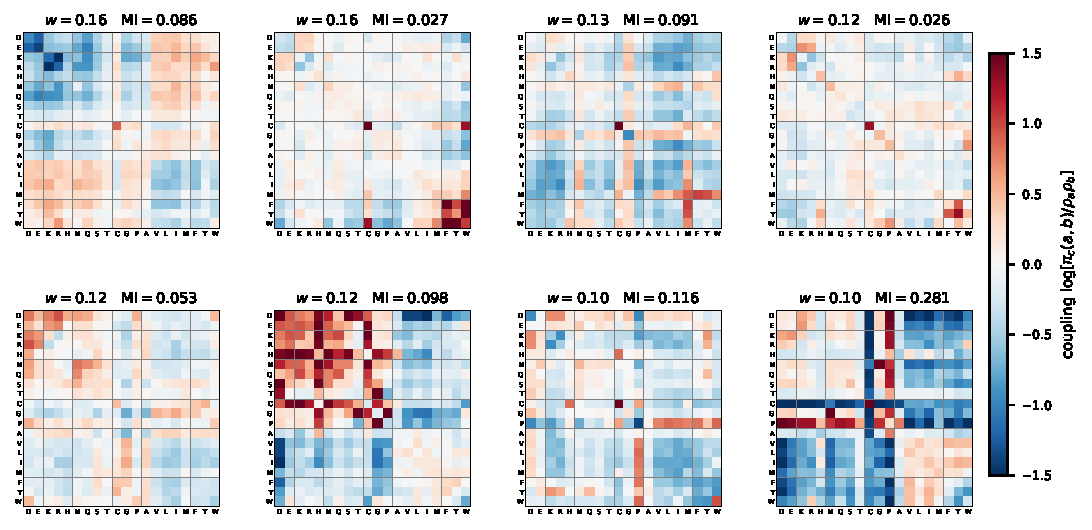
\includegraphics[width=\textwidth]{mixture_components_K8.pdf}
\caption{\textbf{The eight \Metrop-mixture coupling classes ($K{=}8$).} Each panel is
one fitted interaction class's coupling $\log[\pi_c(a,b)/\rho_a\rho_b]$ over the $400$
amino-acid pairs (red favoured, blue disfavoured; $\rho$ is the class marginal). Residues are ordered by group (acidic\,$|$\,basic\,$|$\,polar\,$|$\,special\,$|$\,aliphatic\,$|$\,aromatic).
Panels are sorted by mixture weight $w$ and annotated with the stationary mutual information
$\mathrm{MI}(\pi_c)$. The classes carry coherent but \emph{different} couplings---acid--base
complementarity (the off-diagonal acidic/basic blocks) in some, aliphatic assortativity (the
\texttt{AVLIM} block) in others---so pooling them into one shared chain averages
opposite-sign couplings down to the $0.027$-nat residual (\Cref{tab:axes}). Per-class
fitting keeps each coupling intact.}
\label{fig:components}
\end{figure}

\begin{table}[t]
\caption{Biophysical coupling in trRosetta per-contact tensors. Each axis’s ``pooled'' pair correlation decomposes into ``within''-class and ``between''-classes contributions. All values are standardised to the pooled marginal (unit property
variance). ``Strength'' is the mean per-class $|\mathrm{Cov}_c|$.
``Per-class signs'' reports whether the within-class covariance is positive ($\texttt{+}$), negative ($\texttt{-}$), or near zero ($\texttt{0}$).
Charge is a weaker axis than hydropathy or volume, but it is
the only one whose within-class coupling survives pooling. This is due to 
its largely consistent sign (mostly complementary); hydropathy and volume flip signs across classes and cancel.}
\label{tab:axes}
\centering
\footnotesize
\setlength{\tabcolsep}{6pt}
\begin{tabular}{lrrrrl}
\toprule
Axis & Strength & Within (survives) & Between (comp.) & Pooled & Per-class signs\\
\midrule
Charge      & $0.10$ & $-0.096$ & $+0.014$ & $-0.082$ & \texttt{-{-}-{-}-+-{-}}\\
Hydropathy  & $0.14$ & $-0.013$ & $+0.198$ & $+0.185$ & \texttt{-0++-+-+}\\
Volume      & $0.12$ & $-0.048$ & $+0.118$ & $+0.070$ & \texttt{-+-+-+-+}\\
Aromatic    & $0.05$ & $+0.014$ & $+0.014$ & $+0.028$ & \texttt{-+0+-+-{-}}\\
\bottomrule
\end{tabular}
\end{table}

% =============================================================
\section{Many components and variational inference}
\label{sec:multi}
% =============================================================

The pair models have $A^2$ states, growing to $A^L$ for $L$ coupled sites. Exact
matrix exponentiation does not simplify for the general \CTBN, and Felsenstein's
downward pass breaks the factorization its upward pass keeps.
Existing phylogenetic approaches to this scaling problem use context-dependent chains,
ML/MCMC-EM estimators, and variational or truncation bounds~\cite{ArndtBurgeHwa2003NeighborDependent,ChristensenHobolthJensen2005PseudoLikelihood,Hobolth2008MCMCEM,JensenPedersen2000ContextDependent,JojicEtAl2004PhyloHMM,LunterHein2004NearestNeighbor,MathewsSchmidler2025ImportanceSampling,MatsenRalph2022BoundingDependency,SiepelHaussler2004ContextML,WexlerGeiger2007VariationalUpper}.
We take the variational law to be a product of independent single-site \CTMC\
bridges~\cite{cohn2010}. The bound is written in the bridge statistics~\eqref{eq:bridge} of
the $A^L$ product chain, but these collapse to a boundary term and a one-dimensional
integral over single-site bridge marginals: polynomial, not exponential, in cluster size.

\paragraph{Path ELBO.} Let a cluster of $L$ sites carry the Potts target
$\Pi(x)\propto e^{-E(x)}$, $x\in\Xset^L$, with
$E(x)=-\sum_s h_s(x_s)-\sum_{s<s'}H_{ss'}(x_s,x_{s'})$, and let the independent
single-site GTR proposal $R_{ab}=S_{ab}\pi_b$ act site-wise. Suppose the coupling is carried
by the \emph{square-root}\footnote{
Among acceptances $A(z)\propto z^\theta$, reversibility ($A(z)=zA(1/z)$) forces
$\theta=\tfrac12$: the square root is the unique log-linear reversible acceptance, i.e.\
the only one for which $\log(W/R)$ is a potential difference~\eqref{eq:logWR}.
} \Metrop\ target rate for the move $x\to x^{s:c}$ that replaces
residue $i=x_s$ at site $s$ with $c$,
\begin{equation}\label{eq:sqrtmet}
 W_{x,x^{s:c}}=R_{ic}\sqrt{\tfrac{\Pi(x^{s:c})R_{ci}}{\Pi(x)R_{ic}}}
 =S_{ic}\sqrt{\pi_i\pi_c}\;e^{-\frac12\Delta^c_sE(x)},\qquad
 \Delta^c_sE(x)=E(x^{s:c})-E(x),
\end{equation}
reversible w.r.t.\ $\Pi$ for any $S,h,H$. On a branch of length $t$ with $x(0)=a$, $x(t)=b$,
using the product of independent $R$-chains as a variational proposal\footnote{
As described here, the proposal is fixed; it can be made variational, e.g. by introducing midpoint-node distributions.
},
Girsanov's formula for jump processes writes the log-density ratio of the two path
measures as a difference of \emph{complete-data} log-likelihoods of the
form~\eqref{eq:cdl}: a trajectory $\mathbb X$ with usages $U$ and dwell times $T$ has
\begin{equation}\label{eq:girsanov}
 \log\frac{d\mathbb P_W}{d\mathbb P_R}(\mathbb X)=\ell_W(\mathbb X)-\ell_R(\mathbb X),
 \qquad
 \ell_Q(\mathbb X)=\sum_{x\ne y}U_{xy}\log Q_{xy}-\sum_xT_x\,q(x),
\end{equation}
with $q(x)=\sum_{y\ne x}Q_{xy}$ the exit rate. The ELBO adds the $R$-bridge average of this
difference to the proposal's own log-transition probability,
\begin{equation}\label{eq:pathelbo}
 \mathcal L_{ab}=\log[e^{tR}]_{ab}
 +\sum_{x,s,c\ne x_s}\bar N^{ab}_{x,s:c}\log\frac{W_{x,x^{s:c}}}{R_{x_sc}}
 -\sum_x\bar T^{ab}_x\,[w(x)-r(x)],
\end{equation}
where $w(x)=\sum_{s,c}W_{x,x^{s:c}}$ and $r(x)=\sum_{s,c}R_{x_sc}$ are the two exit rates
and $\bar T,\bar N$ are the dwell and usage bridge statistics~\eqref{eq:bridge} of the
$A^L$-state product chain; Jensen's inequality gives
$\mathcal L_{ab}\le\log[e^{tW}]_{ab}$. The statistics that drive the \EM\ of
\Cref{sec:single} therefore also carry the bound: it is the expected \emph{gain} in
complete-data log-likelihood from replacing the proposal by the coupled target, added to
what the proposal already explains.

Equation~\eqref{eq:pathelbo} is the mean-field free energy of Cohn et
al.~\cite{cohn2010} at one member of their factored family, and is consistent with their Theorem~3:
where Cohn et al. optimise a time-varying \emph{inhomogeneous} rate via Euler-Lagrange ODEs, we consider the product of single-site
bridges of the \emph{time-homogeneous} $R$. Fixing the rates, rather than
solving their ODEs, makes ours the looser of the two bounds, but more stable to compute: the terms that diverge as $u\to t$
(their rate integral divides by a backward probability vanishing at the endpoint)
telescope analytically into the $\log[e^{tR}]_{ab}$ normaliser, leaving a smooth
integrand. The partition function of
$\Pi$ cancels from every rate ratio in \eqref{eq:sqrtmet}, entering only the root factor
of the tree likelihood. Both contractions below rely on log-linearity making the log-rate
ratio a \emph{potential difference},
\begin{equation}\label{eq:logWR}
 \log\frac{W_{x,x^{s:c}}}{R_{x_sc}}=\psi(x^{s:c})-\psi(x),
 \qquad
 \psi(x)=-\tfrac12\sum_s\log\pi_{x_s}-\tfrac12E(x).
\end{equation}

\begin{figure}[t]
\centering
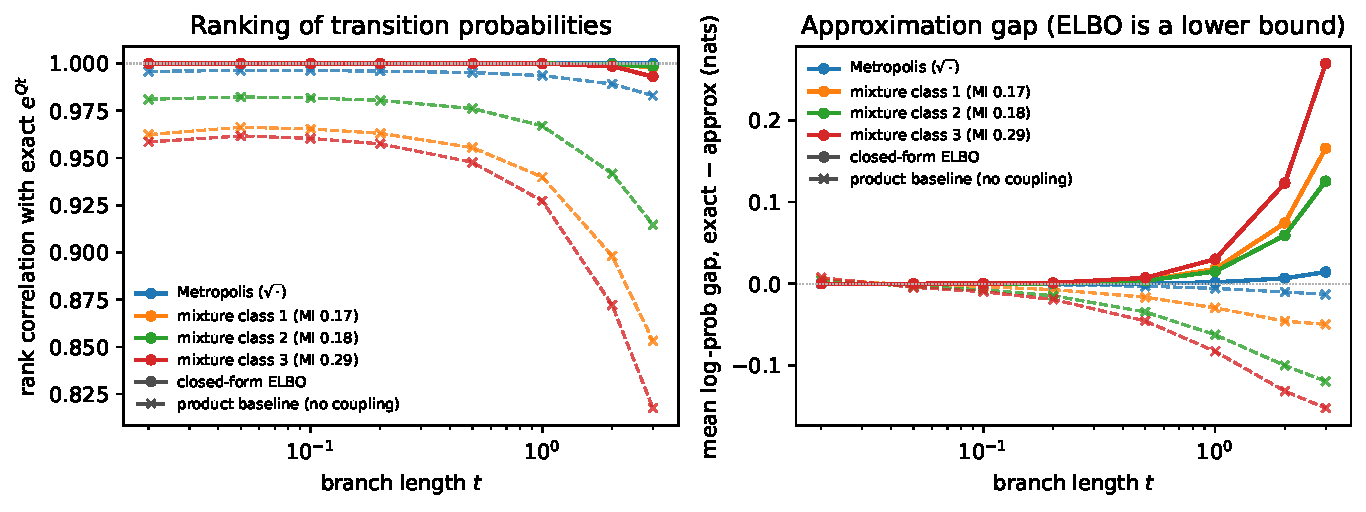
\includegraphics[width=0.78\textwidth]{figures/elbo_vs_expm_combined_legend.pdf}
\caption{\textbf{The path ELBO tracks the exact matrix exponential.} \eqref{eq:pathelbo}
for coupled pairs, where it is exactly closed-form, against exact $[e^{tQ}]$ over branch
length $t$, for the \Metrop\ chain and the three strongest-coupled mixture components.
\emph{Left:} global Spearman between ELBO and exact log-transition entries (solid) stays
$\approx1$, well above the coupling-free product baseline $[e^{tR}]$ (dashed).
\emph{Right:} mean gap exact$-$approx; the ELBO is a lower bound near zero for
$t\lesssim1$, growing at long branches and strong coupling, while the baseline is not a
bound.}
\label{fig:elbovsexpm}
\end{figure}

\paragraph{Contraction to per-site bridge statistics.} The statistics $\bar T,\bar N$ are
joint over $A^L$ and do \emph{not} factorise, but both terms of \eqref{eq:pathelbo}
reduce to per-site quantities, for two different consequences of~\eqref{eq:logWR}.

\emph{The usage term is a boundary term.} Every jump of the product chain moves one site,
so along any path $a=x_0\to\cdots\to x_K=b$ the increments $\psi(x_k)-\psi(x_{k-1})$
telescope to $\psi(b)-\psi(a)$: the same value for every path, whatever its length or
order. Since $\sum_{x,s,c}\bar N^{ab}_{x,s:c}f$ is by definition the bridge
expectation of $\sum_{\mathrm{jumps}}f$, and the expectation of a path-independent
quantity is that quantity,
\begin{equation}\label{eq:telescope}
 \sum_{x,\,s,\,c\ne x_s}\bar N^{ab}_{x,s:c}\log\frac{W_{x,x^{s:c}}}{R_{x_sc}}
 =\tfrac12\sum_s\log\frac{\pi_{a_s}}{\pi_{b_s}}+\tfrac12\big[E(a)-E(b)\big].
\end{equation}

\emph{The dwell term contracts to a one-dimensional integral.} The product chain has
$M_{ab}(t)=\prod_sM^s_{a_sb_s}(t)$, so \eqref{eq:bridge} gives
$\bar T^{ab}_x=\int_0^t\prod_sp^s_u(x_s)\,du$ and hence, for any $\phi$,
\begin{equation}\label{eq:contract}
 \sum_x\bar T^{ab}_x\,\phi(x)=\int_0^t\!\E_u[\phi]\;du,
 \qquad
 p^s_u(y)=\frac{M^s_{a_sy}(u)\,M^s_{yb_s}(t-u)}{M^s_{a_sb_s}(t)},
\end{equation}
with $M^s(u)=e^{uR}$ and $\E_u$ the expectation under the product measure
$\prod_sp^s_u$: the joint sum has become a time integral of an expectation over
\emph{independent} sites. Now $-\tfrac12\Delta^c_sE(x)$ is a sum over the neighbours of
$s$, so $W$ is a \emph{product} over them, and the expectation of a product of functions
of distinct independent sites is the product of the expectations,
\begin{equation}\label{eq:sep}
 \E_u\big[W_{x,x^{s:c}}\big]=\sum_i p^s_u(i)\,S_{ic}\sqrt{\pi_i\pi_c}\;
   e^{\frac12[h_s(c)-h_s(i)]}
   \prod_{s'\ne s}\Big(\sum_z p^{s'}_u(z)\;e^{\frac12[H_{ss'}(c,z)-H_{ss'}(i,z)]}\Big).
\end{equation}
Every factor is a single sum over one site's alphabet, so the $A^L$ configuration sum
never forms, even though the exit rate depends on all neighbours jointly and nonlinearly:
separability across neighbours, not linearity, is what is required. The proposal exit rate
$r$ is one-body and contracts likewise.
At each quadrature node, evaluating \eqref{eq:sep} costs $O(A^3)$ per contact and $O(A^2)$
per site, so the ELBO costs $O\!\big(m(LA^2+|\mathcal C|A^3)\big)$ for $m$ quadrature nodes
and $|\mathcal C|$ contacts (the coupled pairs $s<s'$ with $H_{ss'}\ne0$): polynomial in
cluster size rather than exponential.

\paragraph{When the time integral is exact.} Factorisation across sites is not
factorisation across time, so \eqref{eq:contract} leaves a genuine integral. Each
$p^s_u$ is a sum of $A^2$ exponentials in $u$, so the integrand of \eqref{eq:sep} is a
product of one such sum per coupled site, $L$ in all. For $L=2$ the integral is the
divided-difference kernel~\eqref{eq:bridgestat} and $\mathcal L_{ab}$ is
exactly closed-form---the regime of \Cref{fig:elbovsexpm}. Larger clusters give $A^{2L}$
terms and we integrate numerically instead. Its exponents are those of $R$, so it is
entire and Gauss--Legendre converges spectrally: with $R$ set to LG08, $m\le14$ nodes reach
machine precision for $L\le5$, $t\le3$ and couplings up to $|H|\sim4$. This conditioning separates
the bound from the inhomogeneous mean field, whose endpoint-singular integrand converges
at first order.

The bound is a faithful surrogate for the exact coupled matrix exponential
(\Cref{fig:elbovsexpm}): its mean gap stays close to zero for $t\lesssim1$, and it
preserves the exact transition-probability ranking (global Spearman $\ge0.998$),
consistently above the coupling-free product baseline and by the largest margin at long
branches. Against the mean field of Cohn et al.~\cite{cohn2010} on the same pairs, our
implementation of their ODE system fails to converge on $30$--$40\%$ of pairs at short
branches, and on $\approx41\%$ of the converged ones the returned value exceeds the exact
log-likelihood; their bound is valid by construction, so these are integration errors in
the endpoint boundary layer. Their solver is also $\sim100\times$ slower.


%\paragraph{Stability against the Cohn mean field.} Compared directly to the
%endpoint-conditioned mean field of Cohn et al.~\cite{cohn2010} that it warm-starts
%(\Cref{sec:potts}), the closed form is the more dependable object
%(\Cref{fig:cohngap}): the path ELBO and its single-midpoint refinement are certified
%lower bounds, near-exact for $t\lesssim1$ and tighter still with the midpoint, while the
%full Cohn mean field---whose rate integral has an endpoint singularity---fails to
%converge on up to $30$--$40\%$ of pairs at short branches and, where it does converge,
%violates the bound on $\approx41\%$ of them. It matches Cohn's tightness without the
%ODE stiffness or bound violations, at whole-matrix rather than per-pair-ODE cost.

%\begin{figure}[t]
%\centering
%\includegraphics[width=\textwidth]{cohn_gap.pdf}
%\caption{\textbf{The closed-form ELBO is stable where the Cohn mean field is not.} Mean
%per-pair bound gap (exact $\log[e^{tW}]_{xy}$ minus approximation, nats) versus branch
%length $t$, for the two strongest-coupled \Metrop-mixture classes (stationary mutual
%information $0.16$ and $0.29$), each over $4{,}000$ importance-sampled endpoint pairs per
%branch length (full-$\psi$ Cohn over its converged subset, $\le\!92$ pairs). Curves: the
%closed-form path ELBO \eqref{eq:pathelbo}; its single-midpoint refinement (one interior
%variational node per branch---the first step of the mesh refinement of \Cref{sec:potts});
%and the Cohn mean field with and without the neighbour back-reaction $\psi$ of
%\eqref{eq:girsanov}. All four are lower bounds, so a gap $\ge0$ is required. The grey step
%(right axis) is the fraction of full-$\psi$ Cohn solves that fail to converge within a
%$16{,}384$-step ODE budget; it peaks at short branches, where the endpoint singularity of
%the Cohn rate integral is strongest. Full-$\psi$ Cohn additionally violates the bound
%(gap $<0$) at long branches, on $\approx41\%$ of converged pairs pooled across classes and
%$t$; the closed forms never do. Error bars: gap $\pm1$ SE of the mean; grey band $\pm1$ SE
%(binomial).}
%\label{fig:cohngap}
%\end{figure}

%%% I think this is the only section to drop; re: "Honestly we could probably safely 
%%%   drop the product-of-trees stuff. It doesn't add much"
%Combining the closed-form ELBO above with the product-of-trees variational fit of
%Jojic et al.~\cite{JojicEtAl2004PhyloHMM} gives a method that jointly fits the Potts
%coupling and reconstructs ancestral sequences.
%the same E-step that fits $H$ keeps a
%full along-branch law per site, so it returns the posterior residue distribution at
%every internal node and coevolution-aware ancestral reconstruction is a byproduct.
%We implemented this; it works, but on protein families it returns essentially the same
%reconstructions as independent-site ASR, concordant with prior
%reports~\cite{MunizTrejo2025,ZeinatyEtAl2026ASR}. This matches our other findings in
%tone: amino-acid coupling is a minor effect in protein phylogenetics. The algorithm,
%the phylogenetic fixed-bridge Potts ELBO, is given in the supplementary appendix.



%% =============================================================
%\section{Combining coevolution with indels: the TKF--DP}
%\label{sec:tkfdp}
%% =============================================================
%
%The coupled substitution model supplies the substitution side of an indel
%model. Run TKF92 with indel parameters $(\lambda,\mu,r)$; deal each surviving
%residue, at birth, a key class $z_s$ from the stick-breaking weights of a
%Dirichlet process with concentration $\alpha_z$, so on $L$ sites the induced
%partition is Ewens~\cite{ewens1972,aldous1985} and residues sharing a table are
%coupling partners, with coevolution mediated by a ``shared field'' common to each table.
%This is the TKF Dirichlet process (TKF--DP): TKF92 with site-independence relaxed via de Finetti.
%
%\paragraph{Stationarity implies marginal-consistency.} For a coupled cluster $C$ with joint stationary
%$\pi_C$, the augmented substitution-plus-indel process is reversible at a
%deletion exactly when
%$\sum_{x_s}\pi_C(x_C)=\pi_{C\setminus s}(x_{C\setminus s})$ for every $s\in C$,
%so a residue joining a table draws from the conditional
%$\pi_C(x_s\mid x_{C\setminus s})$ and its later deletion is exact
%marginalisation.
%%Iterated to any observed subset this is the projective
%%Kolmogorov condition. When it holds, the substitution factor detaches from the
%%indel bookkeeping and the alignment marginal is exactly plain TKF92's; when it
%%fails, deleting a covarying partner shifts the survivors' composition and the
%%alignment likelihood picks up a spurious dependence on the coupling. A raw
%%pairwise Potts joint violates \Cref{eq:consistency}, which is why the pair
%%Potts model needs the Sinkhorn repair of \Cref{sec:pair}; the shared field
%%satisfies it by construction, because the members are conditionally independent
%%draws from field-indexed stationaries.
%
%\paragraph{Lumpability confers indifference to ghosts.}
%In order to compute cluster likelihoods under the \TKFDP, we need to account for the possibility of transiently inserted lineages temporarily joining the cluster.
%This requires that the cluster likelihood is lumpable, surviving projection to the observed members.
%This is the motivation for having the coevolution be driven by a latent time-evolving variable associated with the site;
%the observed residues merely reflect the state of this variable.
%This further ensures marginal-consistency, as introduced in the previous paragraph.
%As a practical accommodation, if we limit clusters to two members, we can use any of the models from \Cref{sec:paircompare}.
%
%\paragraph{Alignment: the infinite pair HMM.} The generalization of the TKF92 Pair HMM to the \TKFDP\ is
%an \emph{infinite Pair HMM}~\cite{BealGhahramaniRasmussen2001} whose match states track the Ewens partition.
%We sample the joint posterior over alignments and couplings by MCMC, precomputing partial Forward matrices
%for efficient resampling of alignments between coupling pins.
%
%On the held-out Laminin EGF-like family (\Pfam\ \texttt{PF00053}) the coupled
%sampler recovers the canonical disulfide pattern from sequence alone: the eight
%conserved cysteines generate $28$ candidate Cys--Cys column pairs, and all $28$
%fall within the top $50$ column-pair posteriors, with mean Cys--Cys posterior
%$0.087$ against $0.004$ background, about $22$ times enriched
%(\Cref{fig:pf00053}). These are exactly the coevolving, indel-punctuated
%interactions that a fixed-graph alignment-conditioned Potts model is least
%equipped to recover, because the couplings and the gaps arrive together.
%Using the pairwise posteriors for multiple alignment yields improvements over plain TKF92 in sum-of-pairs (SP) and total-column (TC) accuracy
%(\Cref{tab:aln}).
%The improvement is very slight, perhaps due to the weak coupling signal in pairwise alignments.
%
%\begin{figure}[t]
%\centering
%\includegraphics[width=0.78\textwidth]{holmes_msa_triangle_PF00053_K8.pdf}
%\caption{\textbf{Coupled column-pair posterior on held-out \texttt{PF00053}.}
%All $28$ candidate Cys--Cys pairs fall in the top $50$ posteriors; the non-Cys
%top arcs cluster on the cb-EGF Ca$^{2+}$ pocket and conserved $\beta$-hairpin
%turns.}
%\label{fig:pf00053}
%\end{figure}
%
%\begin{table}[t]
%\caption{Pairwise-alignment accuracy on BAliBASE \texttt{bali3pdbm} ($L{<}150$
%subset, $22$ families / $187$ sequence pairs). For the pair-HMM models (top
%block) the MSA is assembled by feeding pairwise match posteriors into
%FSA~\cite{BradleyEtAl2009}; $F_1$, SP and TC are standard accuracy metrics. CherryML ($C{=}20$) is a $20$-class site mixture fitted by
%CherryML~\cite{Prillo2023CherryML}. MAFFT~\cite{Katoh2013} and
%MUSCLE~\cite{Edgar2004} are shown for reference.}
%\label{tab:aln}
%\centering
%\footnotesize
%\setlength{\tabcolsep}{6pt}
%\begin{tabular}{lccc}
%\toprule
%Method & MSA $F_1$ & SP & TC\\
%\midrule
%TKF92                            & 0.514 & 0.724 & 0.631\\
%TKF92 ($K_c{=}20$)               & 0.515 & 0.732 & 0.637\\
%CherryML ($C{=}20$)              & 0.515 & 0.723 & 0.629\\
%Coupled $K_c{=}8$                & 0.513 & 0.730 & 0.640\\
%\midrule
%MAFFT (FFT-NS-2)                 & 0.509 & 0.691 & 0.558\\
%MUSCLE (default)                 & 0.512 & 0.760 & 0.662\\
%\bottomrule
%\end{tabular}
%\end{table}

% =============================================================
\section{Discussion}
\label{sec:discussion}
% =============================================================

Symmetry is central to molecular evolution: the invariants (reversibility,
exchangeability) of a coupled substitution process inform the design of a coevolutionary
model. We have used them to extend the \EM\ algorithm to coevolutionary substitution
models, and presented a variational approximation for larger clusters.
Locally-correlated rate heterogeneity, needed by models that partition by domain or
secondary structure~\cite{Yang1995,ThorneGoldmanJones96,LargeHolmes2026}, is a natural
complement to this work.

% Do NOT include this section in the anonymized submission, only in the final paper. You can use the \texttt{ack} environment provided in the style file to automatically hide this section in the anonymized submission.
%\begin{ack}
%We thank Debora Marks, Yun Song, and Sebastian Prillo for helpful discussions. Selected mathematical
%derivations and exposition were generated by Anthropic and OpenAI products
%under the supervision of the human authors. The work was funded
%by NIH grants HG004483, GM080203, and HG013117. 
%\end{ack}

%% References follow the acknowledgments and do not count towards the page
%% limit.  natbib+plainnat sets the unnumbered "References" heading itself.
%% The .bib file lives in this directory.
\label{endofbody}
\clearpage
\bibliographystyle{plainnat}
\bibliography{refs}

%%%%%%%%%%%%%%%%%%%%%%%%%%%%%%%%%%%%%%%%%%%%%%%%%%%%%%%%%%%%

\newpage
\section*{NeurIPS Paper Checklist}

%%% BEGIN INSTRUCTIONS %%%
The checklist is designed to encourage best practices for responsible machine learning research, addressing issues of reproducibility, transparency, research ethics, and societal impact. Do not remove the checklist: {\bf The papers not including the checklist will be desk rejected.} The checklist should follow the references and follow the (optional) supplemental material.  The checklist does NOT count towards the page
limit. 

Please read the checklist guidelines carefully for information on how to answer these questions. For each question in the checklist:
\begin{itemize}
    \item You should answer \answerYes{}, \answerNo{}, or \answerNA{}.
    \item \answerNA{} means either that the question is Not Applicable for that particular paper or the relevant information is Not Available.
    \item Please provide a short (1--2 sentence) justification right after your answer (even for \answerNA). 
   % \item {\bf The papers not including the checklist will be desk rejected.}
\end{itemize}

{\bf The checklist answers are an integral part of your paper submission.} They are visible to the reviewers, area chairs, senior area chairs, and ethics reviewers. You will also be asked to include it (after eventual revisions) with the final version of your paper, and its final version will be published with the paper.

The reviewers of your paper will be asked to use the checklist as one of the factors in their evaluation. While \answerYes{} is generally preferable to \answerNo{}, it is perfectly acceptable to answer \answerNo{} provided a proper justification is given (e.g., error bars are not reported because it would be too computationally expensive'' or ``we were unable to find the license for the dataset we used''). In general, answering \answerNo{} or \answerNA{} is not grounds for rejection. While the questions are phrased in a binary way, we acknowledge that the true answer is often more nuanced, so please just use your best judgment and write a justification to elaborate. All supporting evidence can appear either in the main paper or the supplemental material, provided in appendix. If you answer \answerYes{} to a question, in the justification please point to the section(s) where related material for the question can be found.

IMPORTANT, please:
\begin{itemize}
    \item {\bf Delete this instruction block, but keep the section heading ``NeurIPS Paper Checklist"},
    \item  {\bf Keep the checklist subsection headings, questions/answers and guidelines below.}
    \item {\bf Do not modify the questions and only use the provided macros for your answers}.
\end{itemize} 
 

%%% END INSTRUCTIONS %%%


\begin{enumerate}

\item {\bf Claims}
    \item[] Question: Do the main claims made in the abstract and introduction accurately reflect the paper's contributions and scope?
    \item[] Answer: \answerTODO{} % Replace by \answerYes{}, \answerNo{}, or \answerNA{}.
    \item[] Justification: \justificationTODO{}
    \item[] Guidelines:
    \begin{itemize}
        \item The answer \answerNA{} means that the abstract and introduction do not include the claims made in the paper.
        \item The abstract and/or introduction should clearly state the claims made, including the contributions made in the paper and important assumptions and limitations. A \answerNo{} or \answerNA{} answer to this question will not be perceived well by the reviewers. 
        \item The claims made should match theoretical and experimental results, and reflect how much the results can be expected to generalize to other settings. 
        \item It is fine to include aspirational goals as motivation as long as it is clear that these goals are not attained by the paper. 
    \end{itemize}

\item {\bf Limitations}
    \item[] Question: Does the paper discuss the limitations of the work performed by the authors?
    \item[] Answer: \answerTODO{} % Replace by \answerYes{}, \answerNo{}, or \answerNA{}.
    \item[] Justification: \justificationTODO{}
    \item[] Guidelines:
    \begin{itemize}
        \item The answer \answerNA{} means that the paper has no limitation while the answer \answerNo{} means that the paper has limitations, but those are not discussed in the paper. 
        \item The authors are encouraged to create a separate ``Limitations'' section in their paper.
        \item The paper should point out any strong assumptions and how robust the results are to violations of these assumptions (e.g., independence assumptions, noiseless settings, model well-specification, asymptotic approximations only holding locally). The authors should reflect on how these assumptions might be violated in practice and what the implications would be.
        \item The authors should reflect on the scope of the claims made, e.g., if the approach was only tested on a few datasets or with a few runs. In general, empirical results often depend on implicit assumptions, which should be articulated.
        \item The authors should reflect on the factors that influence the performance of the approach. For example, a facial recognition algorithm may perform poorly when image resolution is low or images are taken in low lighting. Or a speech-to-text system might not be used reliably to provide closed captions for online lectures because it fails to handle technical jargon.
        \item The authors should discuss the computational efficiency of the proposed algorithms and how they scale with dataset size.
        \item If applicable, the authors should discuss possible limitations of their approach to address problems of privacy and fairness.
        \item While the authors might fear that complete honesty about limitations might be used by reviewers as grounds for rejection, a worse outcome might be that reviewers discover limitations that aren't acknowledged in the paper. The authors should use their best judgment and recognize that individual actions in favor of transparency play an important role in developing norms that preserve the integrity of the community. Reviewers will be specifically instructed to not penalize honesty concerning limitations.
    \end{itemize}

\item {\bf Theory assumptions and proofs}
    \item[] Question: For each theoretical result, does the paper provide the full set of assumptions and a complete (and correct) proof?
    \item[] Answer: \answerTODO{} % Replace by \answerYes{}, \answerNo{}, or \answerNA{}.
    \item[] Justification: \justificationTODO{}
    \item[] Guidelines:
    \begin{itemize}
        \item The answer \answerNA{} means that the paper does not include theoretical results. 
        \item All the theorems, formulas, and proofs in the paper should be numbered and cross-referenced.
        \item All assumptions should be clearly stated or referenced in the statement of any theorems.
        \item The proofs can either appear in the main paper or the supplemental material, but if they appear in the supplemental material, the authors are encouraged to provide a short proof sketch to provide intuition. 
        \item Inversely, any informal proof provided in the core of the paper should be complemented by formal proofs provided in appendix or supplemental material.
        \item Theorems and Lemmas that the proof relies upon should be properly referenced. 
    \end{itemize}

    \item {\bf Experimental result reproducibility}
    \item[] Question: Does the paper fully disclose all the information needed to reproduce the main experimental results of the paper to the extent that it affects the main claims and/or conclusions of the paper (regardless of whether the code and data are provided or not)?
    \item[] Answer: \answerTODO{} % Replace by \answerYes{}, \answerNo{}, or \answerNA{}.
    \item[] Justification: \justificationTODO{}
    \item[] Guidelines:
    \begin{itemize}
        \item The answer \answerNA{} means that the paper does not include experiments.
        \item If the paper includes experiments, a \answerNo{} answer to this question will not be perceived well by the reviewers: Making the paper reproducible is important, regardless of whether the code and data are provided or not.
        \item If the contribution is a dataset and\slash or model, the authors should describe the steps taken to make their results reproducible or verifiable. 
        \item Depending on the contribution, reproducibility can be accomplished in various ways. For example, if the contribution is a novel architecture, describing the architecture fully might suffice, or if the contribution is a specific model and empirical evaluation, it may be necessary to either make it possible for others to replicate the model with the same dataset, or provide access to the model. In general. releasing code and data is often one good way to accomplish this, but reproducibility can also be provided via detailed instructions for how to replicate the results, access to a hosted model (e.g., in the case of a large language model), releasing of a model checkpoint, or other means that are appropriate to the research performed.
        \item While NeurIPS does not require releasing code, the conference does require all submissions to provide some reasonable avenue for reproducibility, which may depend on the nature of the contribution. For example
        \begin{enumerate}
            \item If the contribution is primarily a new algorithm, the paper should make it clear how to reproduce that algorithm.
            \item If the contribution is primarily a new model architecture, the paper should describe the architecture clearly and fully.
            \item If the contribution is a new model (e.g., a large language model), then there should either be a way to access this model for reproducing the results or a way to reproduce the model (e.g., with an open-source dataset or instructions for how to construct the dataset).
            \item We recognize that reproducibility may be tricky in some cases, in which case authors are welcome to describe the particular way they provide for reproducibility. In the case of closed-source models, it may be that access to the model is limited in some way (e.g., to registered users), but it should be possible for other researchers to have some path to reproducing or verifying the results.
        \end{enumerate}
    \end{itemize}


\item {\bf Open access to data and code}
    \item[] Question: Does the paper provide open access to the data and code, with sufficient instructions to faithfully reproduce the main experimental results, as described in supplemental material?
    \item[] Answer: \answerTODO{} % Replace by \answerYes{}, \answerNo{}, or \answerNA{}.
    \item[] Justification: \justificationTODO{}
    \item[] Guidelines:
    \begin{itemize}
        \item The answer \answerNA{} means that paper does not include experiments requiring code.
        \item Please see the NeurIPS code and data submission guidelines (\url{https://neurips.cc/public/guides/CodeSubmissionPolicy}) for more details.
        \item While we encourage the release of code and data, we understand that this might not be possible, so \answerNo{} is an acceptable answer. Papers cannot be rejected simply for not including code, unless this is central to the contribution (e.g., for a new open-source benchmark).
        \item The instructions should contain the exact command and environment needed to run to reproduce the results. See the NeurIPS code and data submission guidelines (\url{https://neurips.cc/public/guides/CodeSubmissionPolicy}) for more details.
        \item The authors should provide instructions on data access and preparation, including how to access the raw data, preprocessed data, intermediate data, and generated data, etc.
        \item The authors should provide scripts to reproduce all experimental results for the new proposed method and baselines. If only a subset of experiments are reproducible, they should state which ones are omitted from the script and why.
        \item At submission time, to preserve anonymity, the authors should release anonymized versions (if applicable).
        \item Providing as much information as possible in supplemental material (appended to the paper) is recommended, but including URLs to data and code is permitted.
    \end{itemize}


\item {\bf Experimental setting/details}
    \item[] Question: Does the paper specify all the training and test details (e.g., data splits, hyperparameters, how they were chosen, type of optimizer) necessary to understand the results?
    \item[] Answer: \answerTODO{} % Replace by \answerYes{}, \answerNo{}, or \answerNA{}.
    \item[] Justification: \justificationTODO{}
    \item[] Guidelines:
    \begin{itemize}
        \item The answer \answerNA{} means that the paper does not include experiments.
        \item The experimental setting should be presented in the core of the paper to a level of detail that is necessary to appreciate the results and make sense of them.
        \item The full details can be provided either with the code, in appendix, or as supplemental material.
    \end{itemize}

\item {\bf Experiment statistical significance}
    \item[] Question: Does the paper report error bars suitably and correctly defined or other appropriate information about the statistical significance of the experiments?
    \item[] Answer: \answerTODO{} % Replace by \answerYes{}, \answerNo{}, or \answerNA{}.
    \item[] Justification: \justificationTODO{}
    \item[] Guidelines:
    \begin{itemize}
        \item The answer \answerNA{} means that the paper does not include experiments.
        \item The authors should answer \answerYes{} if the results are accompanied by error bars, confidence intervals, or statistical significance tests, at least for the experiments that support the main claims of the paper.
        \item The factors of variability that the error bars are capturing should be clearly stated (for example, train/test split, initialization, random drawing of some parameter, or overall run with given experimental conditions).
        \item The method for calculating the error bars should be explained (closed form formula, call to a library function, bootstrap, etc.)
        \item The assumptions made should be given (e.g., Normally distributed errors).
        \item It should be clear whether the error bar is the standard deviation or the standard error of the mean.
        \item It is OK to report 1-sigma error bars, but one should state it. The authors should preferably report a 2-sigma error bar than state that they have a 96\% CI, if the hypothesis of Normality of errors is not verified.
        \item For asymmetric distributions, the authors should be careful not to show in tables or figures symmetric error bars that would yield results that are out of range (e.g., negative error rates).
        \item If error bars are reported in tables or plots, the authors should explain in the text how they were calculated and reference the corresponding figures or tables in the text.
    \end{itemize}

\item {\bf Experiments compute resources}
    \item[] Question: For each experiment, does the paper provide sufficient information on the computer resources (type of compute workers, memory, time of execution) needed to reproduce the experiments?
    \item[] Answer: \answerTODO{} % Replace by \answerYes{}, \answerNo{}, or \answerNA{}.
    \item[] Justification: \justificationTODO{}
    \item[] Guidelines:
    \begin{itemize}
        \item The answer \answerNA{} means that the paper does not include experiments.
        \item The paper should indicate the type of compute workers CPU or GPU, internal cluster, or cloud provider, including relevant memory and storage.
        \item The paper should provide the amount of compute required for each of the individual experimental runs as well as estimate the total compute. 
        \item The paper should disclose whether the full research project required more compute than the experiments reported in the paper (e.g., preliminary or failed experiments that didn't make it into the paper). 
    \end{itemize}
    
\item {\bf Code of ethics}
    \item[] Question: Does the research conducted in the paper conform, in every respect, with the NeurIPS Code of Ethics \url{https://neurips.cc/public/EthicsGuidelines}?
    \item[] Answer: \answerTODO{} % Replace by \answerYes{}, \answerNo{}, or \answerNA{}.
    \item[] Justification: \justificationTODO{}
    \item[] Guidelines:
    \begin{itemize}
        \item The answer \answerNA{} means that the authors have not reviewed the NeurIPS Code of Ethics.
        \item If the authors answer \answerNo, they should explain the special circumstances that require a deviation from the Code of Ethics.
        \item The authors should make sure to preserve anonymity (e.g., if there is a special consideration due to laws or regulations in their jurisdiction).
    \end{itemize}


\item {\bf Broader impacts}
    \item[] Question: Does the paper discuss both potential positive societal impacts and negative societal impacts of the work performed?
    \item[] Answer: \answerTODO{} % Replace by \answerYes{}, \answerNo{}, or \answerNA{}.
    \item[] Justification: \justificationTODO{}
    \item[] Guidelines:
    \begin{itemize}
        \item The answer \answerNA{} means that there is no societal impact of the work performed.
        \item If the authors answer \answerNA{} or \answerNo, they should explain why their work has no societal impact or why the paper does not address societal impact.
        \item Examples of negative societal impacts include potential malicious or unintended uses (e.g., disinformation, generating fake profiles, surveillance), fairness considerations (e.g., deployment of technologies that could make decisions that unfairly impact specific groups), privacy considerations, and security considerations.
        \item The conference expects that many papers will be foundational research and not tied to particular applications, let alone deployments. However, if there is a direct path to any negative applications, the authors should point it out. For example, it is legitimate to point out that an improvement in the quality of generative models could be used to generate Deepfakes for disinformation. On the other hand, it is not needed to point out that a generic algorithm for optimizing neural networks could enable people to train models that generate Deepfakes faster.
        \item The authors should consider possible harms that could arise when the technology is being used as intended and functioning correctly, harms that could arise when the technology is being used as intended but gives incorrect results, and harms following from (intentional or unintentional) misuse of the technology.
        \item If there are negative societal impacts, the authors could also discuss possible mitigation strategies (e.g., gated release of models, providing defenses in addition to attacks, mechanisms for monitoring misuse, mechanisms to monitor how a system learns from feedback over time, improving the efficiency and accessibility of ML).
    \end{itemize}
    
\item {\bf Safeguards}
    \item[] Question: Does the paper describe safeguards that have been put in place for responsible release of data or models that have a high risk for misuse (e.g., pre-trained language models, image generators, or scraped datasets)?
    \item[] Answer: \answerTODO{} % Replace by \answerYes{}, \answerNo{}, or \answerNA{}.
    \item[] Justification: \justificationTODO{}
    \item[] Guidelines:
    \begin{itemize}
        \item The answer \answerNA{} means that the paper poses no such risks.
        \item Released models that have a high risk for misuse or dual-use should be released with necessary safeguards to allow for controlled use of the model, for example by requiring that users adhere to usage guidelines or restrictions to access the model or implementing safety filters. 
        \item Datasets that have been scraped from the Internet could pose safety risks. The authors should describe how they avoided releasing unsafe images.
        \item We recognize that providing effective safeguards is challenging, and many papers do not require this, but we encourage authors to take this into account and make a best faith effort.
    \end{itemize}

\item {\bf Licenses for existing assets}
    \item[] Question: Are the creators or original owners of assets (e.g., code, data, models), used in the paper, properly credited and are the license and terms of use explicitly mentioned and properly respected?
    \item[] Answer: \answerTODO{} % Replace by \answerYes{}, \answerNo{}, or \answerNA{}.
    \item[] Justification: \justificationTODO{}
    \item[] Guidelines:
    \begin{itemize}
        \item The answer \answerNA{} means that the paper does not use existing assets.
        \item The authors should cite the original paper that produced the code package or dataset.
        \item The authors should state which version of the asset is used and, if possible, include a URL.
        \item The name of the license (e.g., CC-BY 4.0) should be included for each asset.
        \item For scraped data from a particular source (e.g., website), the copyright and terms of service of that source should be provided.
        \item If assets are released, the license, copyright information, and terms of use in the package should be provided. For popular datasets, \url{paperswithcode.com/datasets} has curated licenses for some datasets. Their licensing guide can help determine the license of a dataset.
        \item For existing datasets that are re-packaged, both the original license and the license of the derived asset (if it has changed) should be provided.
        \item If this information is not available online, the authors are encouraged to reach out to the asset's creators.
    \end{itemize}

\item {\bf New assets}
    \item[] Question: Are new assets introduced in the paper well documented and is the documentation provided alongside the assets?
    \item[] Answer: \answerTODO{} % Replace by \answerYes{}, \answerNo{}, or \answerNA{}.
    \item[] Justification: \justificationTODO{}
    \item[] Guidelines:
    \begin{itemize}
        \item The answer \answerNA{} means that the paper does not release new assets.
        \item Researchers should communicate the details of the dataset\slash code\slash model as part of their submissions via structured templates. This includes details about training, license, limitations, etc. 
        \item The paper should discuss whether and how consent was obtained from people whose asset is used.
        \item At submission time, remember to anonymize your assets (if applicable). You can either create an anonymized URL or include an anonymized zip file.
    \end{itemize}

\item {\bf Crowdsourcing and research with human subjects}
    \item[] Question: For crowdsourcing experiments and research with human subjects, does the paper include the full text of instructions given to participants and screenshots, if applicable, as well as details about compensation (if any)? 
    \item[] Answer: \answerTODO{} % Replace by \answerYes{}, \answerNo{}, or \answerNA{}.
    \item[] Justification: \justificationTODO{}
    \item[] Guidelines:
    \begin{itemize}
        \item The answer \answerNA{} means that the paper does not involve crowdsourcing nor research with human subjects.
        \item Including this information in the supplemental material is fine, but if the main contribution of the paper involves human subjects, then as much detail as possible should be included in the main paper. 
        \item According to the NeurIPS Code of Ethics, workers involved in data collection, curation, or other labor should be paid at least the minimum wage in the country of the data collector. 
    \end{itemize}

\item {\bf Institutional review board (IRB) approvals or equivalent for research with human subjects}
    \item[] Question: Does the paper describe potential risks incurred by study participants, whether such risks were disclosed to the subjects, and whether Institutional Review Board (IRB) approvals (or an equivalent approval/review based on the requirements of your country or institution) were obtained?
    \item[] Answer: \answerTODO{} % Replace by \answerYes{}, \answerNo{}, or \answerNA{}.
    \item[] Justification: \justificationTODO{}
    \item[] Guidelines:
    \begin{itemize}
        \item The answer \answerNA{} means that the paper does not involve crowdsourcing nor research with human subjects.
        \item Depending on the country in which research is conducted, IRB approval (or equivalent) may be required for any human subjects research. If you obtained IRB approval, you should clearly state this in the paper. 
        \item We recognize that the procedures for this may vary significantly between institutions and locations, and we expect authors to adhere to the NeurIPS Code of Ethics and the guidelines for their institution. 
        \item For initial submissions, do not include any information that would break anonymity (if applicable), such as the institution conducting the review.
    \end{itemize}

\item {\bf Declaration of LLM usage}
    \item[] Question: Does the paper describe the usage of LLMs if it is an important, original, or non-standard component of the core methods in this research? Note that if the LLM is used only for writing, editing, or formatting purposes and does \emph{not} impact the core methodology, scientific rigor, or originality of the research, declaration is not required.
    %this research? 
    \item[] Answer: \answerTODO{} % Replace by \answerYes{}, \answerNo{}, or \answerNA{}.
    \item[] Justification: \justificationTODO{}
    \item[] Guidelines:
    \begin{itemize}
        \item The answer \answerNA{} means that the core method development in this research does not involve LLMs as any important, original, or non-standard components.
        \item Please refer to our LLM policy in the NeurIPS handbook for what should or should not be described.
    \end{itemize}

\end{enumerate}

\end{document}
